\documentclass[twoside]{book}

% Packages required by doxygen
\usepackage{fixltx2e}
\usepackage{calc}
\usepackage{doxygen}
\usepackage[export]{adjustbox} % also loads graphicx
\usepackage{graphicx}
\usepackage[utf8]{inputenc}
\usepackage{makeidx}
\usepackage{multicol}
\usepackage{multirow}
\PassOptionsToPackage{warn}{textcomp}
\usepackage{textcomp}
\usepackage[nointegrals]{wasysym}
\usepackage[table]{xcolor}

% Font selection
\usepackage[T1]{fontenc}
\usepackage[scaled=.90]{helvet}
\usepackage{courier}
\usepackage{amssymb}
\usepackage{sectsty}
\renewcommand{\familydefault}{\sfdefault}
\allsectionsfont{%
  \fontseries{bc}\selectfont%
  \color{darkgray}%
}
\renewcommand{\DoxyLabelFont}{%
  \fontseries{bc}\selectfont%
  \color{darkgray}%
}
\newcommand{\+}{\discretionary{\mbox{\scriptsize$\hookleftarrow$}}{}{}}

% Page & text layout
\usepackage{geometry}
\geometry{%
  a4paper,%
  top=2.5cm,%
  bottom=2.5cm,%
  left=2.5cm,%
  right=2.5cm%
}
\tolerance=750
\hfuzz=15pt
\hbadness=750
\setlength{\emergencystretch}{15pt}
\setlength{\parindent}{0cm}
\setlength{\parskip}{3ex plus 2ex minus 2ex}
\makeatletter
\renewcommand{\paragraph}{%
  \@startsection{paragraph}{4}{0ex}{-1.0ex}{1.0ex}{%
    \normalfont\normalsize\bfseries\SS@parafont%
  }%
}
\renewcommand{\subparagraph}{%
  \@startsection{subparagraph}{5}{0ex}{-1.0ex}{1.0ex}{%
    \normalfont\normalsize\bfseries\SS@subparafont%
  }%
}
\makeatother

% Headers & footers
\usepackage{fancyhdr}
\pagestyle{fancyplain}
\fancyhead[LE]{\fancyplain{}{\bfseries\thepage}}
\fancyhead[CE]{\fancyplain{}{}}
\fancyhead[RE]{\fancyplain{}{\bfseries\leftmark}}
\fancyhead[LO]{\fancyplain{}{\bfseries\rightmark}}
\fancyhead[CO]{\fancyplain{}{}}
\fancyhead[RO]{\fancyplain{}{\bfseries\thepage}}
\fancyfoot[LE]{\fancyplain{}{}}
\fancyfoot[CE]{\fancyplain{}{}}
\fancyfoot[RE]{\fancyplain{}{\bfseries\scriptsize Generated by Doxygen }}
\fancyfoot[LO]{\fancyplain{}{\bfseries\scriptsize Generated by Doxygen }}
\fancyfoot[CO]{\fancyplain{}{}}
\fancyfoot[RO]{\fancyplain{}{}}
\renewcommand{\footrulewidth}{0.4pt}
\renewcommand{\chaptermark}[1]{%
  \markboth{#1}{}%
}
\renewcommand{\sectionmark}[1]{%
  \markright{\thesection\ #1}%
}

% Indices & bibliography
\usepackage{natbib}
\usepackage[titles]{tocloft}
\setcounter{tocdepth}{3}
\setcounter{secnumdepth}{5}
\makeindex

% Hyperlinks (required, but should be loaded last)
\usepackage{ifpdf}
\ifpdf
  \usepackage[pdftex,pagebackref=true]{hyperref}
\else
  \usepackage[ps2pdf,pagebackref=true]{hyperref}
\fi
\hypersetup{%
  colorlinks=true,%
  linkcolor=blue,%
  citecolor=blue,%
  unicode%
}

% Custom commands
\newcommand{\clearemptydoublepage}{%
  \newpage{\pagestyle{empty}\cleardoublepage}%
}

\usepackage{caption}
\captionsetup{labelsep=space,justification=centering,font={bf},singlelinecheck=off,skip=4pt,position=top}

%===== C O N T E N T S =====

\begin{document}

% Titlepage & ToC
\hypersetup{pageanchor=false,
             bookmarksnumbered=true,
             pdfencoding=unicode
            }
\pagenumbering{roman}
\begin{titlepage}
\vspace*{7cm}
\begin{center}%
{\Large My Project }\\
\vspace*{1cm}
{\large Generated by Doxygen 1.8.11}\\
\end{center}
\end{titlepage}
\clearemptydoublepage
\tableofcontents
\clearemptydoublepage
\pagenumbering{arabic}
\hypersetup{pageanchor=true}

%--- Begin generated contents ---
\chapter{Class Index}
\section{Class List}
Here are the classes, structs, unions and interfaces with brief descriptions\+:\begin{DoxyCompactList}
\item\contentsline{section}{\hyperlink{structnode}{node} }{\pageref{structnode}}{}
\item\contentsline{section}{\hyperlink{structnode1}{node1} }{\pageref{structnode1}}{}
\item\contentsline{section}{\hyperlink{structnode__info}{node\+\_\+info} }{\pageref{structnode__info}}{}
\end{DoxyCompactList}

\chapter{File Index}
\section{File List}
Here is a list of all files with brief descriptions\+:\begin{DoxyCompactList}
\item\contentsline{section}{\hyperlink{Lab1_8c}{Lab1.\+c} }{\pageref{Lab1_8c}}{}
\end{DoxyCompactList}

\chapter{Class Documentation}
\hypertarget{classList}{}\section{List Class Reference}
\label{classList}\index{List@{List}}


Collaboration diagram for List\+:
\nopagebreak
\begin{figure}[H]
\begin{center}
\leavevmode
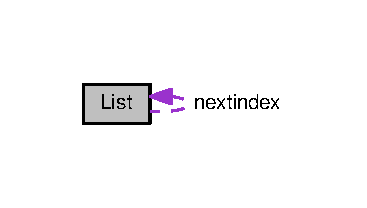
\includegraphics[width=182pt]{classList__coll__graph}
\end{center}
\end{figure}
\subsection*{Classes}
\begin{DoxyCompactItemize}
\item 
struct \hyperlink{structList_1_1Node}{Node}
\end{DoxyCompactItemize}
\subsection*{Public Member Functions}
\begin{DoxyCompactItemize}
\item 
\hyperlink{classList_a06e2fd0daed0264a70fb70194e7d93b6}{List} (\hyperlink{classFruit}{Fruit} $\ast$a\+Fruit)
\item 
\hyperlink{classList_a70aecf37bd9d779a394e4d50377fbf5f}{$\sim$\+List} ()
\item 
void \hyperlink{classList_aa38578a39e87e4b5d349d50e179dfa7a}{append} (\hyperlink{classFruit}{Fruit} $\ast$a\+Fruit)
\item 
void \hyperlink{classList_a1bb66c2777061ab3b8260746a8c3961e}{print\+List} ()
\end{DoxyCompactItemize}
\subsection*{Private Attributes}
\begin{DoxyCompactItemize}
\item 
\hyperlink{structList_1_1Node}{Node} $\ast$ \hyperlink{classList_a443db628080a04a1dacfd3015d164735}{head}
\item 
\hyperlink{structList_1_1Node}{Node} $\ast$ \hyperlink{classList_ac35bbbb4a3103f9574e74491d52dbeba}{tail}
\end{DoxyCompactItemize}


\subsection{Constructor \& Destructor Documentation}
\index{List@{List}!List@{List}}
\index{List@{List}!List@{List}}
\subsubsection[{\texorpdfstring{List(\+Fruit $\ast$a\+Fruit)}{List(Fruit *aFruit)}}]{\setlength{\rightskip}{0pt plus 5cm}List\+::\+List (
\begin{DoxyParamCaption}
\item[{{\bf Fruit} $\ast$}]{a\+Fruit}
\end{DoxyParamCaption}
)\hspace{0.3cm}{\ttfamily [inline]}}\hypertarget{classList_a06e2fd0daed0264a70fb70194e7d93b6}{}\label{classList_a06e2fd0daed0264a70fb70194e7d93b6}

\begin{DoxyCode}
59 \{\hyperlink{classList_a443db628080a04a1dacfd3015d164735}{head} = \hyperlink{classList_ac35bbbb4a3103f9574e74491d52dbeba}{tail} = \textcolor{keyword}{new} Node(aFruit); \}
\end{DoxyCode}
\index{List@{List}!````~List@{$\sim$\+List}}
\index{````~List@{$\sim$\+List}!List@{List}}
\subsubsection[{\texorpdfstring{$\sim$\+List()}{~List()}}]{\setlength{\rightskip}{0pt plus 5cm}List\+::$\sim$\+List (
\begin{DoxyParamCaption}
{}
\end{DoxyParamCaption}
)\hspace{0.3cm}{\ttfamily [inline]}}\hypertarget{classList_a70aecf37bd9d779a394e4d50377fbf5f}{}\label{classList_a70aecf37bd9d779a394e4d50377fbf5f}

\begin{DoxyCode}
61             \{
62         \textcolor{keywordflow}{while} (\hyperlink{classList_a443db628080a04a1dacfd3015d164735}{head} != NULL)\{             \textcolor{comment}{// traverse list deallocating memory}
63            Node* save = \hyperlink{classList_a443db628080a04a1dacfd3015d164735}{head};
64            \hyperlink{classList_a443db628080a04a1dacfd3015d164735}{head} = \hyperlink{classList_a443db628080a04a1dacfd3015d164735}{head}->\hyperlink{structList_1_1Node_a0e9bd3ca8dc4c1307c04ecb2250fdada}{next};
65            \textcolor{keyword}{delete} save->\hyperlink{structList_1_1Node_a0014e96ae0a971590091f68233a8de2f}{fruitPtr};  save->fruitPtr = NULL;
66            \textcolor{keyword}{delete} save;  save = NULL;
67         \}
68         \hyperlink{classList_ac35bbbb4a3103f9574e74491d52dbeba}{tail} = NULL;
69      \}
\end{DoxyCode}


\subsection{Member Function Documentation}
\index{List@{List}!append@{append}}
\index{append@{append}!List@{List}}
\subsubsection[{\texorpdfstring{append(\+Fruit $\ast$a\+Fruit)}{append(Fruit *aFruit)}}]{\setlength{\rightskip}{0pt plus 5cm}void List\+::append (
\begin{DoxyParamCaption}
\item[{{\bf Fruit} $\ast$}]{a\+Fruit}
\end{DoxyParamCaption}
)\hspace{0.3cm}{\ttfamily [inline]}}\hypertarget{classList_aa38578a39e87e4b5d349d50e179dfa7a}{}\label{classList_aa38578a39e87e4b5d349d50e179dfa7a}

\begin{DoxyCode}
71                                \{          \textcolor{comment}{// append at end of list}
72        \hyperlink{classList_ac35bbbb4a3103f9574e74491d52dbeba}{tail}->\hyperlink{structList_1_1Node_a0e9bd3ca8dc4c1307c04ecb2250fdada}{next} = \textcolor{keyword}{new} Node(aFruit);                             
73        \hyperlink{classList_ac35bbbb4a3103f9574e74491d52dbeba}{tail} = \hyperlink{classList_ac35bbbb4a3103f9574e74491d52dbeba}{tail}->\hyperlink{structList_1_1Node_a0e9bd3ca8dc4c1307c04ecb2250fdada}{next};
74     \}
\end{DoxyCode}
\index{List@{List}!print\+List@{print\+List}}
\index{print\+List@{print\+List}!List@{List}}
\subsubsection[{\texorpdfstring{print\+List()}{printList()}}]{\setlength{\rightskip}{0pt plus 5cm}void List\+::print\+List (
\begin{DoxyParamCaption}
{}
\end{DoxyParamCaption}
)\hspace{0.3cm}{\ttfamily [inline]}}\hypertarget{classList_a1bb66c2777061ab3b8260746a8c3961e}{}\label{classList_a1bb66c2777061ab3b8260746a8c3961e}

\begin{DoxyCode}
76                      \{                    \textcolor{comment}{// traverse list printing}
77        \textcolor{keywordflow}{for} (Node* p = \hyperlink{classList_a443db628080a04a1dacfd3015d164735}{head}; p != NULL; p = p->\hyperlink{structList_1_1Node_a0e9bd3ca8dc4c1307c04ecb2250fdada}{next})
78           p->fruitPtr->print();
79     \}
\end{DoxyCode}


\subsection{Member Data Documentation}
\index{List@{List}!head@{head}}
\index{head@{head}!List@{List}}
\subsubsection[{\texorpdfstring{head}{head}}]{\setlength{\rightskip}{0pt plus 5cm}{\bf Node}$\ast$ List\+::head\hspace{0.3cm}{\ttfamily [private]}}\hypertarget{classList_a443db628080a04a1dacfd3015d164735}{}\label{classList_a443db628080a04a1dacfd3015d164735}
\index{List@{List}!tail@{tail}}
\index{tail@{tail}!List@{List}}
\subsubsection[{\texorpdfstring{tail}{tail}}]{\setlength{\rightskip}{0pt plus 5cm}{\bf Node} $\ast$ List\+::tail\hspace{0.3cm}{\ttfamily [private]}}\hypertarget{classList_ac35bbbb4a3103f9574e74491d52dbeba}{}\label{classList_ac35bbbb4a3103f9574e74491d52dbeba}


The documentation for this class was generated from the following file\+:\begin{DoxyCompactItemize}
\item 
\hyperlink{Fruit_8cpp}{Fruit.\+cpp}\end{DoxyCompactItemize}

\hypertarget{classSparseArray}{}\section{Sparse\+Array Class Reference}
\label{classSparseArray}\index{Sparse\+Array@{Sparse\+Array}}


Collaboration diagram for Sparse\+Array\+:
\nopagebreak
\begin{figure}[H]
\begin{center}
\leavevmode
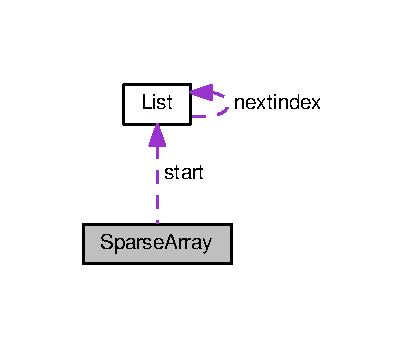
\includegraphics[width=196pt]{classSparseArray__coll__graph}
\end{center}
\end{figure}
\subsection*{Public Member Functions}
\begin{DoxyCompactItemize}
\item 
\hyperlink{classSparseArray_a5c8fafe693c3954efcd607026fa97beb}{Sparse\+Array} (int \hyperlink{classSparseArray_af5a1db82e35f728926e98d3301a29130}{index})
\item 
void \hyperlink{classSparseArray_a9950c0e59ecf391266e1031863b18984}{store} (int \hyperlink{classSparseArray_af5a1db82e35f728926e98d3301a29130}{index}, int value)
\item 
int \hyperlink{classSparseArray_a818714dcef93b33775bdca60b99e97d7}{fetch} (int \hyperlink{classSparseArray_af5a1db82e35f728926e98d3301a29130}{index})
\item 
int \hyperlink{classSparseArray_a73aa431df6e8d5dfeea682d9e2016acd}{element\+Count} ()
\end{DoxyCompactItemize}
\subsection*{Private Attributes}
\begin{DoxyCompactItemize}
\item 
\hyperlink{classList}{List} $\ast$ \hyperlink{classSparseArray_a57186d34f863d9aeb8fb8b9979db63c5}{start}
\item 
int \hyperlink{classSparseArray_af5a1db82e35f728926e98d3301a29130}{index}
\end{DoxyCompactItemize}


\subsection{Constructor \& Destructor Documentation}
\index{Sparse\+Array@{Sparse\+Array}!Sparse\+Array@{Sparse\+Array}}
\index{Sparse\+Array@{Sparse\+Array}!Sparse\+Array@{Sparse\+Array}}
\subsubsection[{\texorpdfstring{Sparse\+Array(int index)}{SparseArray(int index)}}]{\setlength{\rightskip}{0pt plus 5cm}Sparse\+Array\+::\+Sparse\+Array (
\begin{DoxyParamCaption}
\item[{int}]{index}
\end{DoxyParamCaption}
)\hspace{0.3cm}{\ttfamily [inline]}}\hypertarget{classSparseArray_a5c8fafe693c3954efcd607026fa97beb}{}\label{classSparseArray_a5c8fafe693c3954efcd607026fa97beb}

\begin{DoxyCode}
99         \{
100             \hyperlink{classSparseArray_a57186d34f863d9aeb8fb8b9979db63c5}{start} = \textcolor{keyword}{new} \hyperlink{classList}{List}();
101             this->\hyperlink{classSparseArray_af5a1db82e35f728926e98d3301a29130}{index} = \hyperlink{classSparseArray_af5a1db82e35f728926e98d3301a29130}{index};
102         \}
\end{DoxyCode}


\subsection{Member Function Documentation}
\index{Sparse\+Array@{Sparse\+Array}!element\+Count@{element\+Count}}
\index{element\+Count@{element\+Count}!Sparse\+Array@{Sparse\+Array}}
\subsubsection[{\texorpdfstring{element\+Count()}{elementCount()}}]{\setlength{\rightskip}{0pt plus 5cm}int Sparse\+Array\+::element\+Count (
\begin{DoxyParamCaption}
{}
\end{DoxyParamCaption}
)\hspace{0.3cm}{\ttfamily [inline]}}\hypertarget{classSparseArray_a73aa431df6e8d5dfeea682d9e2016acd}{}\label{classSparseArray_a73aa431df6e8d5dfeea682d9e2016acd}

\begin{DoxyCode}
126         \{
127             \textcolor{keywordflow}{return} \hyperlink{classSparseArray_a57186d34f863d9aeb8fb8b9979db63c5}{start}->\hyperlink{classList_a5ee9aff9e61a566f7ce0ac9c6153cda5}{elementCount}();
128         \}
\end{DoxyCode}


Here is the call graph for this function\+:
\nopagebreak
\begin{figure}[H]
\begin{center}
\leavevmode
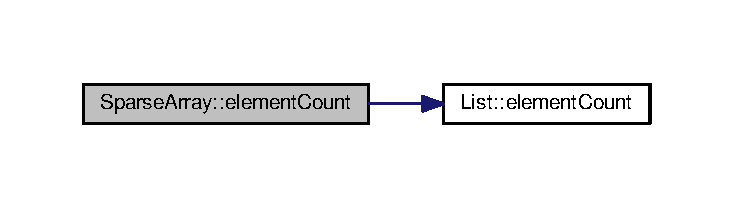
\includegraphics[width=350pt]{classSparseArray_a73aa431df6e8d5dfeea682d9e2016acd_cgraph}
\end{center}
\end{figure}


\index{Sparse\+Array@{Sparse\+Array}!fetch@{fetch}}
\index{fetch@{fetch}!Sparse\+Array@{Sparse\+Array}}
\subsubsection[{\texorpdfstring{fetch(int index)}{fetch(int index)}}]{\setlength{\rightskip}{0pt plus 5cm}int Sparse\+Array\+::fetch (
\begin{DoxyParamCaption}
\item[{int}]{index}
\end{DoxyParamCaption}
)\hspace{0.3cm}{\ttfamily [inline]}}\hypertarget{classSparseArray_a818714dcef93b33775bdca60b99e97d7}{}\label{classSparseArray_a818714dcef93b33775bdca60b99e97d7}

\begin{DoxyCode}
116         \{
117             \textcolor{keywordflow}{if} (\hyperlink{classSparseArray_af5a1db82e35f728926e98d3301a29130}{index} >= 0 && index < this->\hyperlink{classSparseArray_af5a1db82e35f728926e98d3301a29130}{index})
118                 \textcolor{keywordflow}{return} \hyperlink{classSparseArray_a57186d34f863d9aeb8fb8b9979db63c5}{start}->\hyperlink{classList_a7c24ac131f6731a4909424cde96064d0}{fetch}(index);
119             \textcolor{keywordflow}{else} 
120             \{
121                 cout<<\textcolor{stringliteral}{"INDEX OUT OF BOUNDS"}<<endl;
122                 \textcolor{keywordflow}{return} NULL;
123             \}
124         \}
\end{DoxyCode}


Here is the call graph for this function\+:
\nopagebreak
\begin{figure}[H]
\begin{center}
\leavevmode
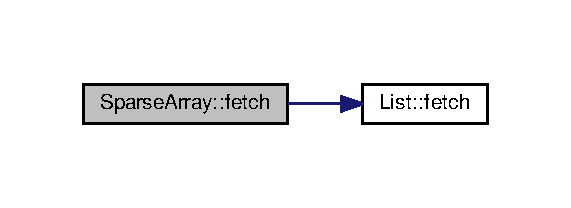
\includegraphics[width=274pt]{classSparseArray_a818714dcef93b33775bdca60b99e97d7_cgraph}
\end{center}
\end{figure}


\index{Sparse\+Array@{Sparse\+Array}!store@{store}}
\index{store@{store}!Sparse\+Array@{Sparse\+Array}}
\subsubsection[{\texorpdfstring{store(int index, int value)}{store(int index, int value)}}]{\setlength{\rightskip}{0pt plus 5cm}void Sparse\+Array\+::store (
\begin{DoxyParamCaption}
\item[{int}]{index, }
\item[{int}]{value}
\end{DoxyParamCaption}
)\hspace{0.3cm}{\ttfamily [inline]}}\hypertarget{classSparseArray_a9950c0e59ecf391266e1031863b18984}{}\label{classSparseArray_a9950c0e59ecf391266e1031863b18984}

\begin{DoxyCode}
104         \{
105             \textcolor{keywordflow}{if} (\hyperlink{classSparseArray_af5a1db82e35f728926e98d3301a29130}{index} >= 0 && index < this->\hyperlink{classSparseArray_af5a1db82e35f728926e98d3301a29130}{index})
106             \{
107                 \textcolor{keywordflow}{if} (value != NULL)
108                     \hyperlink{classSparseArray_a57186d34f863d9aeb8fb8b9979db63c5}{start}->\hyperlink{classList_ae769414aa9a0fc3374df51f3b787c5e9}{store}(index, value);
109             \} 
110             \textcolor{keywordflow}{else}
111             \{
112                 cout<<\textcolor{stringliteral}{"INDEX OUT OF BOUNDS"}<<endl;
113             \}
114         \}
\end{DoxyCode}


Here is the call graph for this function\+:
\nopagebreak
\begin{figure}[H]
\begin{center}
\leavevmode
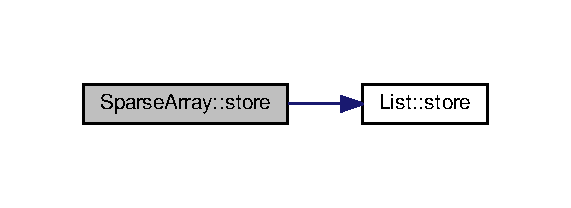
\includegraphics[width=274pt]{classSparseArray_a9950c0e59ecf391266e1031863b18984_cgraph}
\end{center}
\end{figure}




\subsection{Member Data Documentation}
\index{Sparse\+Array@{Sparse\+Array}!index@{index}}
\index{index@{index}!Sparse\+Array@{Sparse\+Array}}
\subsubsection[{\texorpdfstring{index}{index}}]{\setlength{\rightskip}{0pt plus 5cm}int Sparse\+Array\+::index\hspace{0.3cm}{\ttfamily [private]}}\hypertarget{classSparseArray_af5a1db82e35f728926e98d3301a29130}{}\label{classSparseArray_af5a1db82e35f728926e98d3301a29130}
\index{Sparse\+Array@{Sparse\+Array}!start@{start}}
\index{start@{start}!Sparse\+Array@{Sparse\+Array}}
\subsubsection[{\texorpdfstring{start}{start}}]{\setlength{\rightskip}{0pt plus 5cm}{\bf List}$\ast$ Sparse\+Array\+::start\hspace{0.3cm}{\ttfamily [private]}}\hypertarget{classSparseArray_a57186d34f863d9aeb8fb8b9979db63c5}{}\label{classSparseArray_a57186d34f863d9aeb8fb8b9979db63c5}


The documentation for this class was generated from the following file\+:\begin{DoxyCompactItemize}
\item 
\hyperlink{SparseMatrix_8cpp}{Sparse\+Matrix.\+cpp}\end{DoxyCompactItemize}

\hypertarget{classSparseMatrix}{}\section{Sparse\+Matrix Class Reference}
\label{classSparseMatrix}\index{Sparse\+Matrix@{Sparse\+Matrix}}


Collaboration diagram for Sparse\+Matrix\+:
\nopagebreak
\begin{figure}[H]
\begin{center}
\leavevmode
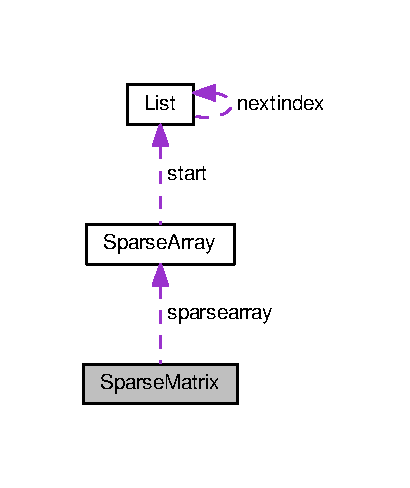
\includegraphics[width=197pt]{classSparseMatrix__coll__graph}
\end{center}
\end{figure}
\subsection*{Public Member Functions}
\begin{DoxyCompactItemize}
\item 
\hyperlink{classSparseMatrix_aa4635499909974beecdcf753342a0f15}{Sparse\+Matrix} (int \hyperlink{classSparseMatrix_a4295e15f08092c633480eff6527918ab}{N})
\item 
void \hyperlink{classSparseMatrix_a4e3b9721dcd31b6db675ab1fba2a83a3}{store} (int rowindex, int colindex, int value)
\item 
int \hyperlink{classSparseMatrix_a2e75c91152fd4f552b010b11aa04a6df}{get} (int rowindex, int colindex)
\item 
int \hyperlink{classSparseMatrix_ab81c07a21a8a25c953d9bd37773da4ee}{element\+Count} ()
\end{DoxyCompactItemize}
\subsection*{Private Attributes}
\begin{DoxyCompactItemize}
\item 
int \hyperlink{classSparseMatrix_a4295e15f08092c633480eff6527918ab}{N}
\item 
\hyperlink{classSparseArray}{Sparse\+Array} $\ast$$\ast$ \hyperlink{classSparseMatrix_a20f42dd05e85c614190cd5c61c478ea0}{sparsearray}
\end{DoxyCompactItemize}


\subsection{Constructor \& Destructor Documentation}
\index{Sparse\+Matrix@{Sparse\+Matrix}!Sparse\+Matrix@{Sparse\+Matrix}}
\index{Sparse\+Matrix@{Sparse\+Matrix}!Sparse\+Matrix@{Sparse\+Matrix}}
\subsubsection[{\texorpdfstring{Sparse\+Matrix(int N)}{SparseMatrix(int N)}}]{\setlength{\rightskip}{0pt plus 5cm}Sparse\+Matrix\+::\+Sparse\+Matrix (
\begin{DoxyParamCaption}
\item[{int}]{N}
\end{DoxyParamCaption}
)\hspace{0.3cm}{\ttfamily [inline]}}\hypertarget{classSparseMatrix_aa4635499909974beecdcf753342a0f15}{}\label{classSparseMatrix_aa4635499909974beecdcf753342a0f15}

\begin{DoxyCode}
140         \{
141             this->\hyperlink{classSparseMatrix_a4295e15f08092c633480eff6527918ab}{N} = \hyperlink{classSparseMatrix_a4295e15f08092c633480eff6527918ab}{N};
142             \hyperlink{classSparseMatrix_a20f42dd05e85c614190cd5c61c478ea0}{sparsearray} = \textcolor{keyword}{new} \hyperlink{classSparseArray}{SparseArray}* [\hyperlink{classSparseMatrix_a4295e15f08092c633480eff6527918ab}{N}];
143             \textcolor{keywordflow}{for} (\textcolor{keywordtype}{int} index = 0; index < \hyperlink{classSparseMatrix_a4295e15f08092c633480eff6527918ab}{N}; index++)
144             \{
145                 \hyperlink{classSparseMatrix_a20f42dd05e85c614190cd5c61c478ea0}{sparsearray}[index] = \textcolor{keyword}{new} \hyperlink{classSparseArray}{SparseArray}(N);
146             \}
147         \}
\end{DoxyCode}


\subsection{Member Function Documentation}
\index{Sparse\+Matrix@{Sparse\+Matrix}!element\+Count@{element\+Count}}
\index{element\+Count@{element\+Count}!Sparse\+Matrix@{Sparse\+Matrix}}
\subsubsection[{\texorpdfstring{element\+Count()}{elementCount()}}]{\setlength{\rightskip}{0pt plus 5cm}int Sparse\+Matrix\+::element\+Count (
\begin{DoxyParamCaption}
{}
\end{DoxyParamCaption}
)\hspace{0.3cm}{\ttfamily [inline]}}\hypertarget{classSparseMatrix_ab81c07a21a8a25c953d9bd37773da4ee}{}\label{classSparseMatrix_ab81c07a21a8a25c953d9bd37773da4ee}

\begin{DoxyCode}
178         \{
179             \textcolor{keywordtype}{int} count = 0;
180             \textcolor{keywordflow}{for} (\textcolor{keywordtype}{int} index = 0; index < \hyperlink{classSparseMatrix_a4295e15f08092c633480eff6527918ab}{N}; index++)
181             \{
182                 count += \hyperlink{classSparseMatrix_a20f42dd05e85c614190cd5c61c478ea0}{sparsearray}[index]->\hyperlink{classSparseArray_a73aa431df6e8d5dfeea682d9e2016acd}{elementCount}();
183             \}
184             \textcolor{keywordflow}{return} count;
185         \}
\end{DoxyCode}


Here is the call graph for this function\+:
\nopagebreak
\begin{figure}[H]
\begin{center}
\leavevmode
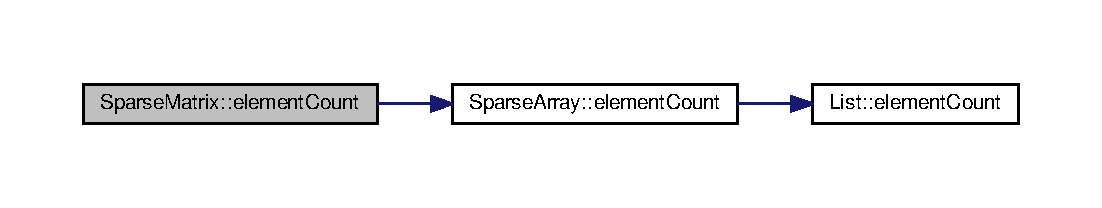
\includegraphics[width=350pt]{classSparseMatrix_ab81c07a21a8a25c953d9bd37773da4ee_cgraph}
\end{center}
\end{figure}


\index{Sparse\+Matrix@{Sparse\+Matrix}!get@{get}}
\index{get@{get}!Sparse\+Matrix@{Sparse\+Matrix}}
\subsubsection[{\texorpdfstring{get(int rowindex, int colindex)}{get(int rowindex, int colindex)}}]{\setlength{\rightskip}{0pt plus 5cm}int Sparse\+Matrix\+::get (
\begin{DoxyParamCaption}
\item[{int}]{rowindex, }
\item[{int}]{colindex}
\end{DoxyParamCaption}
)\hspace{0.3cm}{\ttfamily [inline]}}\hypertarget{classSparseMatrix_a2e75c91152fd4f552b010b11aa04a6df}{}\label{classSparseMatrix_a2e75c91152fd4f552b010b11aa04a6df}

\begin{DoxyCode}
164         \{
165             \textcolor{keywordflow}{if} (rowindex < 0 || colindex > \hyperlink{classSparseMatrix_a4295e15f08092c633480eff6527918ab}{N})
166             \{
167                 cout<<\textcolor{stringliteral}{"row index out of bounds"}<<endl;
168                 \textcolor{keywordflow}{return} 0;
169             \}
170             \textcolor{keywordflow}{if} (rowindex < 0 || colindex > N)
171             \{
172                 cout<<\textcolor{stringliteral}{"col index out of bounds"}<<endl;
173                 \textcolor{keywordflow}{return} 0;
174             \}
175             \textcolor{keywordflow}{return} (\hyperlink{classSparseMatrix_a20f42dd05e85c614190cd5c61c478ea0}{sparsearray}[rowindex]->fetch(colindex));
176         \}
\end{DoxyCode}
\index{Sparse\+Matrix@{Sparse\+Matrix}!store@{store}}
\index{store@{store}!Sparse\+Matrix@{Sparse\+Matrix}}
\subsubsection[{\texorpdfstring{store(int rowindex, int colindex, int value)}{store(int rowindex, int colindex, int value)}}]{\setlength{\rightskip}{0pt plus 5cm}void Sparse\+Matrix\+::store (
\begin{DoxyParamCaption}
\item[{int}]{rowindex, }
\item[{int}]{colindex, }
\item[{int}]{value}
\end{DoxyParamCaption}
)\hspace{0.3cm}{\ttfamily [inline]}}\hypertarget{classSparseMatrix_a4e3b9721dcd31b6db675ab1fba2a83a3}{}\label{classSparseMatrix_a4e3b9721dcd31b6db675ab1fba2a83a3}

\begin{DoxyCode}
149         \{
150             \textcolor{keywordflow}{if} (rowindex < 0 || rowindex > \hyperlink{classSparseMatrix_a4295e15f08092c633480eff6527918ab}{N})
151             \{
152                 cout<<\textcolor{stringliteral}{"row index out of bounds"}<<endl;
153                 \textcolor{keywordflow}{return};
154             \}
155             \textcolor{keywordflow}{if} (colindex < 0 || colindex > N)
156             \{
157                 cout<<\textcolor{stringliteral}{"col index out of bounds"}<<endl;
158                 \textcolor{keywordflow}{return};
159             \}
160             \hyperlink{classSparseMatrix_a20f42dd05e85c614190cd5c61c478ea0}{sparsearray}[rowindex]->\hyperlink{classSparseArray_a9950c0e59ecf391266e1031863b18984}{store}(colindex, value);
161         \}
\end{DoxyCode}


Here is the call graph for this function\+:
\nopagebreak
\begin{figure}[H]
\begin{center}
\leavevmode
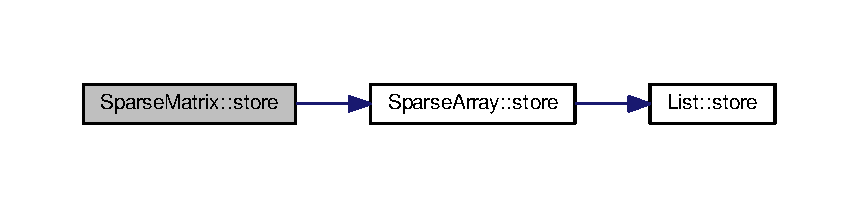
\includegraphics[width=350pt]{classSparseMatrix_a4e3b9721dcd31b6db675ab1fba2a83a3_cgraph}
\end{center}
\end{figure}




\subsection{Member Data Documentation}
\index{Sparse\+Matrix@{Sparse\+Matrix}!N@{N}}
\index{N@{N}!Sparse\+Matrix@{Sparse\+Matrix}}
\subsubsection[{\texorpdfstring{N}{N}}]{\setlength{\rightskip}{0pt plus 5cm}int Sparse\+Matrix\+::N\hspace{0.3cm}{\ttfamily [private]}}\hypertarget{classSparseMatrix_a4295e15f08092c633480eff6527918ab}{}\label{classSparseMatrix_a4295e15f08092c633480eff6527918ab}
\index{Sparse\+Matrix@{Sparse\+Matrix}!sparsearray@{sparsearray}}
\index{sparsearray@{sparsearray}!Sparse\+Matrix@{Sparse\+Matrix}}
\subsubsection[{\texorpdfstring{sparsearray}{sparsearray}}]{\setlength{\rightskip}{0pt plus 5cm}{\bf Sparse\+Array}$\ast$$\ast$ Sparse\+Matrix\+::sparsearray\hspace{0.3cm}{\ttfamily [private]}}\hypertarget{classSparseMatrix_a20f42dd05e85c614190cd5c61c478ea0}{}\label{classSparseMatrix_a20f42dd05e85c614190cd5c61c478ea0}


The documentation for this class was generated from the following file\+:\begin{DoxyCompactItemize}
\item 
\hyperlink{SparseMatrix_8cpp}{Sparse\+Matrix.\+cpp}\end{DoxyCompactItemize}

\chapter{File Documentation}
\hypertarget{SparseMatrix_8cpp}{}\section{Sparse\+Matrix.\+cpp File Reference}
\label{SparseMatrix_8cpp}\index{Sparse\+Matrix.\+cpp@{Sparse\+Matrix.\+cpp}}
{\ttfamily \#include $<$iostream$>$}\\*
{\ttfamily \#include $<$iomanip$>$}\\*
{\ttfamily \#include $<$string$>$}\\*
Include dependency graph for Sparse\+Matrix.\+cpp\+:
\nopagebreak
\begin{figure}[H]
\begin{center}
\leavevmode
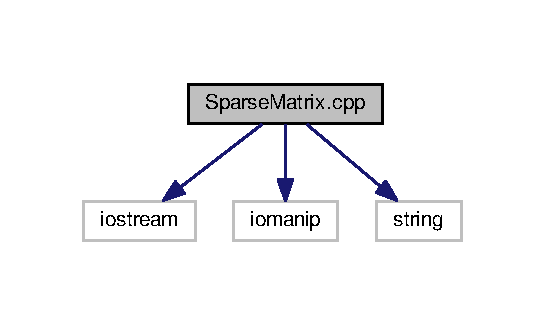
\includegraphics[width=262pt]{SparseMatrix_8cpp__incl}
\end{center}
\end{figure}
\subsection*{Classes}
\begin{DoxyCompactItemize}
\item 
class \hyperlink{classList}{List}
\item 
class \hyperlink{classSparseArray}{Sparse\+Array}
\item 
class \hyperlink{classSparseMatrix}{Sparse\+Matrix}
\end{DoxyCompactItemize}
\subsection*{Functions}
\begin{DoxyCompactItemize}
\item 
int \hyperlink{SparseMatrix_8cpp_ae66f6b31b5ad750f1fe042a706a4e3d4}{main} ()
\end{DoxyCompactItemize}


\subsection{Function Documentation}
\index{Sparse\+Matrix.\+cpp@{Sparse\+Matrix.\+cpp}!main@{main}}
\index{main@{main}!Sparse\+Matrix.\+cpp@{Sparse\+Matrix.\+cpp}}
\subsubsection[{\texorpdfstring{main()}{main()}}]{\setlength{\rightskip}{0pt plus 5cm}int main (
\begin{DoxyParamCaption}
{}
\end{DoxyParamCaption}
)}\hypertarget{SparseMatrix_8cpp_ae66f6b31b5ad750f1fe042a706a4e3d4}{}\label{SparseMatrix_8cpp_ae66f6b31b5ad750f1fe042a706a4e3d4}

\begin{DoxyCode}
191 \{
192     \textcolor{keywordtype}{int} iarray[3][3];
193     iarray[0][0] = 1;
194     iarray[0][1] = NULL;
195     iarray[0][2] = 2;
196     iarray[1][0] = NULL;
197     iarray[1][1] = 3;
198     iarray[1][2] = NULL;
199     iarray[2][0] = 4;
200     iarray[2][1] = 6;
201     iarray[2][2] = NULL;
202     \hyperlink{classSparseMatrix}{SparseMatrix} sparseMatrix(3);
203     \textcolor{keywordflow}{for} (\textcolor{keywordtype}{int} rowindex = 0; rowindex < 3; rowindex++)
204     \{
205         \textcolor{keywordflow}{for} (\textcolor{keywordtype}{int} colindex = 0; colindex < 3; colindex++)
206         \{
207             sparseMatrix.store(rowindex, colindex, iarray[rowindex][colindex]);
208         \}
209     \}
210  
211     cout<<\textcolor{stringliteral}{"the sparse Matrix is: "}<<endl;
212     \textcolor{keywordflow}{for} (\textcolor{keywordtype}{int} rowindex = 0; rowindex < 3; rowindex++)
213     \{
214         \textcolor{keywordflow}{for} (\textcolor{keywordtype}{int} colindex = 0; colindex < 3; colindex++)
215         \{
216             \textcolor{keywordflow}{if} (sparseMatrix.get(rowindex, colindex) == NULL)
217                 cout<<\textcolor{stringliteral}{"NULL"}<< \textcolor{stringliteral}{"\(\backslash\)t"};
218             \textcolor{keywordflow}{else}
219                 cout<<sparseMatrix.get(rowindex, colindex) << \textcolor{stringliteral}{"\(\backslash\)t"};
220         \}
221         cout<<endl;
222     \}
223     cout<<\textcolor{stringliteral}{"The Size of Sparse Matrix is "}<<sparseMatrix.elementCount()<<endl;
224  
225 \}\end{DoxyCode}


Here is the call graph for this function\+:
\nopagebreak
\begin{figure}[H]
\begin{center}
\leavevmode
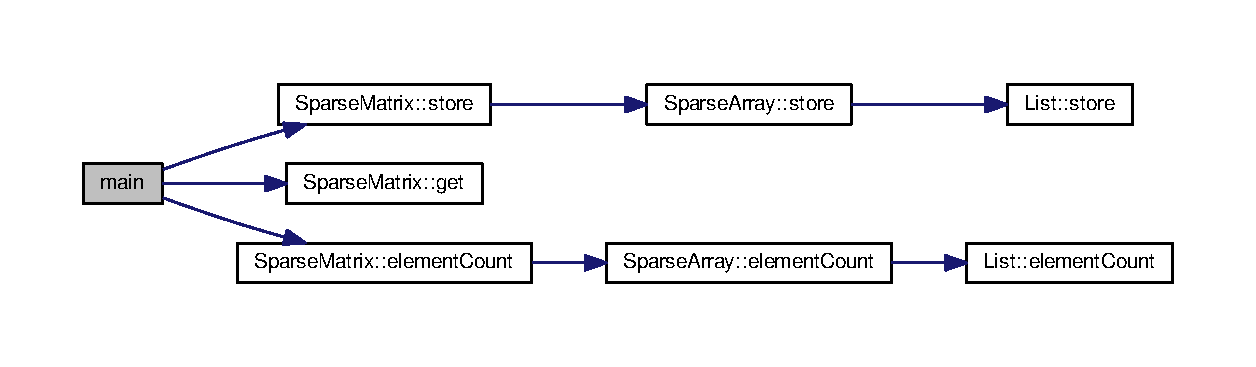
\includegraphics[width=350pt]{SparseMatrix_8cpp_ae66f6b31b5ad750f1fe042a706a4e3d4_cgraph}
\end{center}
\end{figure}



%--- End generated contents ---

% Index
\backmatter
\newpage
\phantomsection
\clearemptydoublepage
\addcontentsline{toc}{chapter}{Index}
\printindex

\end{document}
